\header{5}
\chapter{Reglementen \& Voorrangsregels}
\section{Inleiding}
In dit hoofdstuk wordt gekeken naar de regels en wetten op het water. Op de meeste Nederlandse vaarwateren geldt het Binnenvaart Politie Reglement, het BPR. Het BPR bevat alle regels over de omgang met andere schepen op het water. De belangrijkste delen van het BPR worden in dit hoofdstuk toegelicht

\section{Algemene bepalingen}
Om het BPR goed te kunnen begrijpen, worden eerst een aantal algemene zaken toegelicht. Deze zijn van belang om de regels van het BPR goed te kunnen interpreteren.

Het is verplicht voor alle schepen om een bijgewerkt exemplaar van het BPR bij zich te hebben. Een elektronisch exemplaar wat op ieder moment geraadpleegd kan worden is ook toegestaan. Een uitzondering op deze verplichting geldt voor kleine open schepen. 

\subsection{Type Schepen}
Het BPR maakt onderscheid tussen een aantal verschillende type schepen. De belangrijkste zijn in de onderstaande lijst opgesomd.
\begin{itemize}
	\item \textbf{Schip:} Een schip is een vaartuig geschikt voor vervoer over het water.
    \item \textbf{Motorschip:} Een schip dat mechanische middelen (motor) gebruikt om zich voort te bewegen.
    \item \textbf{Zeilschip:} Een schip dat \textbf{alleen} zijn zeilen gebruikt om voort te bewegen. Een zeilschip dat zijn motor aan heeft wordt gecategoriseerd als een motorschip.
    \item \textbf{Zeilplank:} Een klein zeilschip met een zeil wat in alle richtingen draaibaar is en niet in een vaste positie ondersteund wordt.
    \item \textbf{Passagiersschip:} Een schip dat meer dan 12 personen mag vervoeren. Een passagiersschip kleiner dan 20 meter draagt overdag een gele ruit achter op het schip om dit aan te duiden. 
    \item \textbf{Veerpont:} Een schip dat een veerdienst draait en daarbij een vaarwater oversteekt. \footnote{Dit schip dient daarnaast door de bevoegde autoriteit aangemerkt te worden als veerpont}
    \item \textbf{Klein schip:} Alle schepen onder de 20 meter, met uitzondering van: passagiersschip, veerpont, visser, sleepboot
(alleen als deze grote schepen sleept), duwboot en duwbak. Deze uitzonderingen zijn voor het BPR gelijkwaardig aan grote schepen. 
    \item \textbf{Groot schip:} Schepen groter dan 20 meter, inclusief de eerdergenoemde uitzonderingen. 
    \item \textbf{Sleep:} Een sleep is een samenstel van één of meer motorschepen die andere schepen voorttrekt. 
\end{itemize}

\newpage
\subsection{Termen}
	\begin{itemize}
		\item \textbf{Assisteren:} Assisteren is het bijstaan door een motorschip van een alleen varend motorschip of duwbak bij het sturen of voortbewegen.
		\item \textbf{'s Nachts:} De tijd tussen zonsondergang en zonsopgang.
		\item \textbf{Overdag:} Overdag is de tijd tussen zonsopgang en zonsondergang.
		\item \textbf{Vaarweg:} Een vaarweg is een voor elk openbaar verkeer openstaand water.
		\item \textbf{Vaarwater:} Het gedeelte van de vaarweg dat feitelijk door de scheepvaart wordt  gebruikt.
	\end{itemize}

\subsection{Goed zeemanschap}
Het goed zeemanschap is een hele belangrijke regel op het water. Deze regel houdt in dat de schipper bij het ontbreken van duidelijke regels \textbf{alle nodige voorzorgsmaatregelen} moet nemen om de veiligheid te garanderen, schade te voorkomen of de doorstroom op het water te versoepelen. Ook mag een schipper voor eigen veiligheid of die van anderen afwijken van het BPR.


\subsection{Minimale leeftijden}
Afhankelijk van de snelheid en grootte van een schip gelden er in sommige gevallen minimale leeftijden om een schip te besturen. In de tabel \ref{tab:leeftijd} staan de minimumleeftijden opgesomd. 

\begin{table}[h]
	\centering
	\caption{Minimale leeftijd voor het besturen van een schip}
	\label{tab:leeftijd}
	\begin{tabular}{l|l}
		\textbf{Schip} & \textbf{Minimale Leeftijd} \\ \hline
		Roei- en zeilschip kleiner dan 7 meter			& geen leeftijd \\
		Klein \textit{open} motorschip korter dan 7 meter en maximaal 13 km/h & 12 jaar \\
		Klein motorschip korter dan 7 meter en maximaal 13 km/h & 16 jaar \\
		Groot schip en een zeilschip van meer dan 7 meter & 16 jaar \\
		Snel motorschip ( > 20 km/h) of waterscooter & 18 jaar
		
	\end{tabular}
\end{table}
Een toevoeging op het varen met een snel motorschip en waterscooter is dat hierbij tevens het Klein Vaarbewijs (KVB) I of II vereist is afhankelijk van het vaarwater.

\subsection{Benaming schepen}
Ieder schip, met uitzondering van door spierkracht voortbewogen schepen of zeilschepen kleiner dan 7 meter, dient duidelijk leesbaar de naam van het schip op de buitenzijden te hebben staan.

\subsection{Andere reglementen}
Het BPR geldt niet op \textit{alle} wateren in Nederland. Het is verstandig om vooraf (als je op voor jou onbekende wateren gaat varen) uit te zoeken welke regels er gelden. Dit kan bijvoorbeeld met de ANWB Wateralmanak Deel I.

\subsection{Zwemmen}
Bij het zwemmen is het belangrijk voldoende afstand te houden van varende of drijvende voorwerpen. Mede om deze reden is het verboden te zwemmen is de volgende gebieden:
\begin{itemize}
	\begin{multicols}{2}
		\item Op een wachtplaats van een brug, sluis \\ of stuw
		\item In de vaarweg voor scheepvaart
		\item In de routes van een veerpont 
		\item In havens en nabij de havenmonding
		\item In de nabijheid van aanlegplekken
		\item In gebieden die zijn aangewezen voor snelvaren of waterskiën
		\item In de door autoriteiten aangewezen gebieden
	\end{multicols}
\end{itemize}

\newpage
\section{Voorrangsregels}
Voorrangssituaties zijn te verdelen in drie types: kruisende koersen, tegengestelde koersen en oplopende koersen. Deze koersen zijn te zien in figuur \ref{pic:voorrangkoers}. Welke van deze situaties je vaart bepaalt met welke voorrangsregels je te maken hebt. 
\begin{figure}[H]
    \centering
    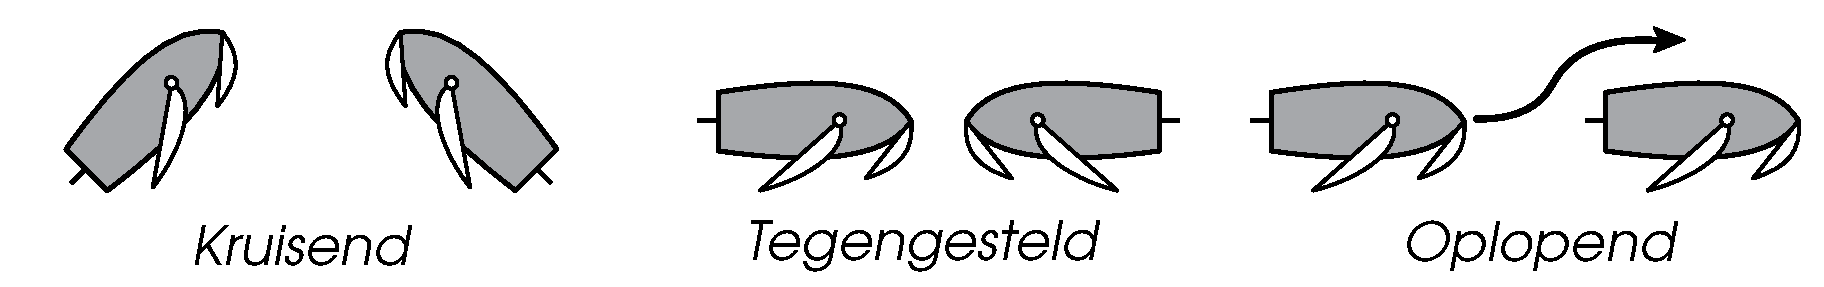
\includegraphics[width=0.8\textwidth]{Hoofdstukken/Reglementen/pdf/voorrangskoersen.pdf}
    \caption{Voorrangskoersen}
    \centering
    \label{pic:voorrangkoers}
\end{figure}
\vspace{-0.4cm}
De voorrangsregels hebben ook een volgorde. Na het bepalen van welke koers je vaart, kijk je altijd eerst naar de bovenste regel die hierbij hoort. Als deze regel niet van toepassing is, ga je pas door naar de volgende. Dit doe je net zo lang tot er een regel is die toe te passen is op jouw situatie.
\paragraph{Kruisende koersen}
\vspace{-0.7cm}
\begin{figure}[H]
	\centering
	\begin{minipage}[t]{0.70\textwidth}
		\textbf{1.} Het schip wat aan de stuurboordswal vaart heeft voorrang.\\
		\textit{Zeilschip A vaart aan de stuurboordswal en heeft voorrang op B}
	\end{minipage}
	\hfill
	\begin{minipage}[t]{0.20\textwidth}
		\raisebox{-0.5\height}{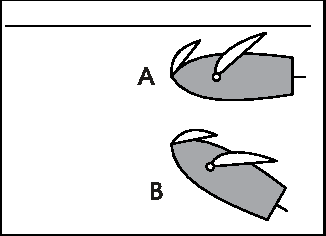
\includegraphics[width=\textwidth]{Hoofdstukken/Reglementen/pdf/kruis_stuurboordswal.pdf}}
		\label{pic:kr1}
	\end{minipage}
	\hfill
\end{figure}

\vspace{-0.7cm}

\begin{figure}[H]
	\centering
	\begin{minipage}[t]{0.70\textwidth}
		\textbf{2.} Grote schepen hebben voorrang op kleine schepen.\\
		\textit{Het grote motorschip A heeft voorrang op het kleine motorschip B}
	\end{minipage}
	\hfill
	\begin{minipage}[t]{0.20\textwidth}
		\raisebox{-0.5\height}{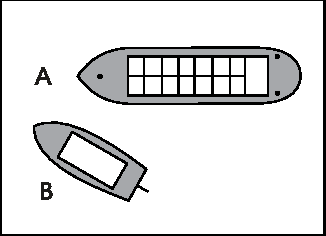
\includegraphics[width=\textwidth]{Hoofdstukken/Reglementen/pdf/kruis_groot_klein.pdf}}	
		\label{pic:kr2}
	\end{minipage}
	\hfill
\end{figure}

\vspace{-0.7cm}
\begin{figure}[H]
	\centering
	\begin{minipage}[t]{0.72\textwidth}
		\textbf{3.} Schepen op het hoofdvaarwater gaan voor op het nevenvaarwater.\\
		\textit{Motorschip A op het hoofddvaarwater heeft voorrang op motorschip B}
	\end{minipage}
	\hfill
	\begin{minipage}[t]{0.20\textwidth}
		\raisebox{-0.5\height}{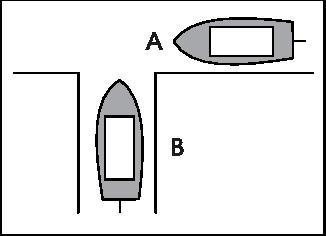
\includegraphics[width=\textwidth]{Hoofdstukken/Reglementen/pdf/kruis_hoofd_neven.pdf}}	
		\label{pic:kr3}
	\end{minipage}
	\hfill
\end{figure}

\vspace{-0.7cm}
\begin{figure}[H]
	\centering
	\begin{minipage}[t]{0.70\textwidth}
		\textbf{4.} Een zeilschip gaat voor een roeiboot gaat voor een motorschip.\\
		\textit{Zeilschip A heeft voorrang op roeiboot B en motorschip C\\
			Roeiboot B heeft voorrang op motorschip C}
	\end{minipage}
	\hfill
	\begin{minipage}[t]{0.20\textwidth}
		\raisebox{-0.65\height}{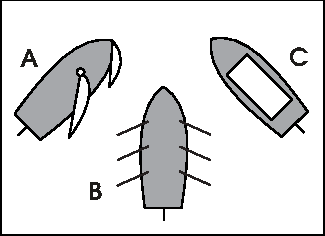
\includegraphics[width=\textwidth]{Hoofdstukken/Reglementen/pdf/kruis_zsm.pdf}}	
		\label{pic:kr4}
	\end{minipage}
	\hfill
\end{figure}

\vspace{-0.7cm}
\begin{figure}[H]
	\centering
	\begin{minipage}[t]{0.70\textwidth}
		\textbf{5.} Motor- en roeiboten onderling: Het schip van rechts gaat voor.\\
		\textit{Motorschip A op rechts heeft voorrang op motorschip B}
	\end{minipage}
	\hfill
	\begin{minipage}[t]{0.20\textwidth}
		\raisebox{-0.65\height}{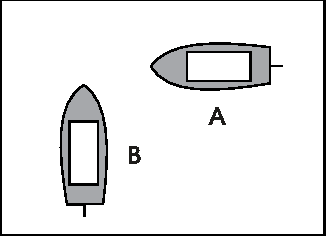
\includegraphics[width=\textwidth]{Hoofdstukken/Reglementen/pdf/kruis_motor_onderling.pdf}}	
		\label{pic:kr5}
	\end{minipage}
	\hfill
\end{figure}

\vspace{-0.7cm}

\textbf{6.} Bij zeilschepen onderling zijn de volgende twee regels van belang:
\vspace{-0.5cm}
\begin{figure}[H]
	\centering
	\hspace{0.02\textwidth}
	\begin{minipage}[t]{0.70\textwidth}
		\textbf{6.1}. Een zeilschip met zeilen over bakboord heeft voorrang.\\
		\textit{Zeilschip B (met zijn zeilen over bakboord) heeft voorrang op \\zeilschip A (met zijn zeilen over stuurboord)}
	\end{minipage}
	\hfill
	\begin{minipage}[t]{0.20\textwidth}
		\raisebox{-0.6\height}{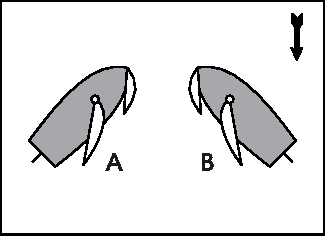
\includegraphics[width=\textwidth]{Hoofdstukken/Reglementen/pdf/kruis_zeilboot_onderling_bakboord.pdf}}	
		\label{pic:kr41}
	\end{minipage}
	\hfill
\end{figure}

\vspace{-0.7cm}
\begin{figure}[H]
	\centering
	\hspace{0.02\textwidth}
	\begin{minipage}[t]{0.70\textwidth}
		\textbf{6.2.} Een zeilschip aan loef wijkt voor een zeilschip aan lij.\\
		\textit{Zeilschip A ligt aan loef van zeilschip B en verleent dus voorrang}
	\end{minipage}
	\hfill
	\begin{minipage}[t]{0.20\textwidth}
		\raisebox{-0.55\height}{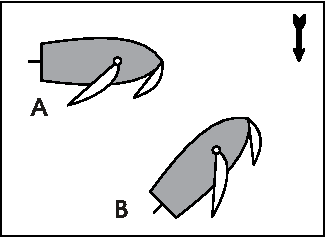
\includegraphics[width=\textwidth]{Hoofdstukken/Reglementen/pdf/kruis_zeilboot_onderling_loef_lij.pdf}}	
		\label{pic:kr42}
	\end{minipage}
	\hfill
\end{figure}


\paragraph{Tegengestelde koersen}
\vspace{-0.2cm}
\begin{figure}[H]
	\centering
	\begin{minipage}[t]{0.70\textwidth}
		\textbf{1.} Het schip wat aan de stuurboordswal vaart heeft voorrang.\\
		\textit{Zeilschip B vaart aan de stuurboordswal en heeft voorrang op A}
	\end{minipage}
	\hfill
	\begin{minipage}[t]{0.25\textwidth}
		\raisebox{-0.55\height}{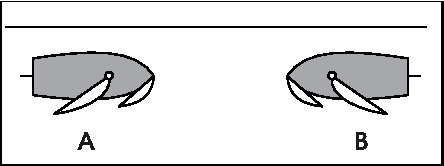
\includegraphics[width=\textwidth]{Hoofdstukken/Reglementen/pdf/tegen_stuurboord.pdf}}
		\label{pic:tg1}
	\end{minipage}
	\hfill
\end{figure}
\vspace{-0.7cm}

\begin{figure}[H]
	\centering
	\begin{minipage}[t]{0.70\textwidth}
		\textbf{2.} Grote schepen hebben voorrang op kleine schepen.\\
		\textit{Het grote motorschip B heeft voorrang op het kleine motorschip A}
	\end{minipage}
	\hfill
	\begin{minipage}[t]{0.25\textwidth}
		\raisebox{-0.55\height}{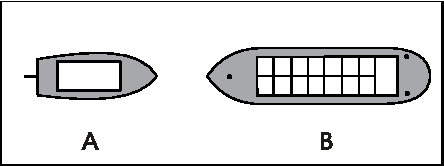
\includegraphics[width=\textwidth]{Hoofdstukken/Reglementen/pdf/tegen_groot_klein.pdf}}
		\label{pic:tg2}
	\end{minipage}
	\hfill
\end{figure}
\vspace{-0.7cm}

\begin{figure}[H]
	\centering
	\begin{minipage}[t]{0.70\textwidth}
		\textbf{3.} Een zeilschip gaat voor een roeiboot gaat voor een motorschip.\\
		\textit{Zeilschip A heeft voorrang op roeiboot B \\
				Zeilschip C heeft voorrang op motorschip D \\
				Roeiboot E heeft voorrang op motorschip F}
	\end{minipage}
	\hfill
	\begin{minipage}[t]{0.25\textwidth}
		\raisebox{-0.75\height}{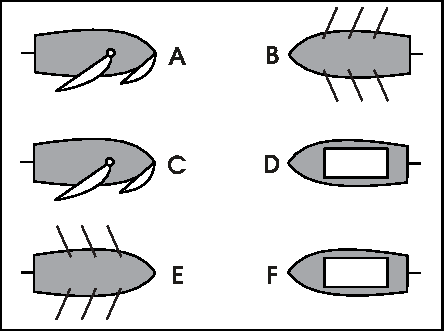
\includegraphics[width=\textwidth]{Hoofdstukken/Reglementen/pdf/tegen_zsm.pdf}}
		\label{pic:tg3a}
	\end{minipage}
	\hfill
\end{figure}
\vspace{-0.7cm}

\begin{figure}[H]
	\centering
	\begin{minipage}[t]{0.70\textwidth}
		\textbf{4.} Zeilschepen onderling: Een zeilschip met zeilen over bakboord heeft voorrang.\\
		\textit{Zeilschip B (met zijn zeilen over bakboord) heeft voorrang op A}
	\end{minipage}
	\hfill
	\begin{minipage}[t]{0.25\textwidth}
		\raisebox{-0.75\height}{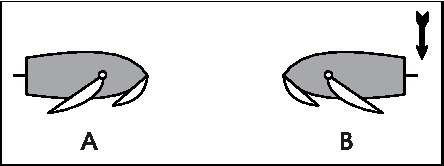
\includegraphics[width=\textwidth]{Hoofdstukken/Reglementen/pdf/tegen_zeilboot_onderling.pdf}}	
		\label{pic:tg4}
	\end{minipage}
	\hfill
\end{figure}
\vspace{-0.7cm}

\begin{figure}[H]
	\centering
	\begin{minipage}[t]{0.70\textwidth}
		\textbf{5.} Roei- of motorschepen onderling: Beide wijken naar bakboord.\\
		\textit{Beide motorschepen wijken naar bakboord}
	\end{minipage}
	\hfill
	\begin{minipage}[t]{0.25\textwidth}
		\raisebox{-0.55\height}{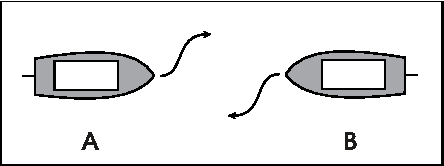
\includegraphics[width=\textwidth]{Hoofdstukken/Reglementen/pdf/tegen_motor_spier_onderling.pdf}}	
		\label{pic:tg5}
	\end{minipage}
	\hfill
\end{figure}

\paragraph{Tegengestelde koersen met engte}
Een engte is een versmalling in het vaarwater waardoor twee schepen niet tegelijk kunnen passeren. Engtes kunnen bijvoorbeeld ontstaan door keringen, open sluizen of het natuurlijk verloop van het water. Bij tegengestelde koersen met engtes gelden de volgende regels:

\begin{figure}[H]
	\centering
	\begin{minipage}[t]{0.70\textwidth}
		\textbf{1.} Bij stroming heeft een schip wat met de stroom mee vaart voorrang.\\
		\textit{Het motorschip A (stroom mee) heeft voorrang op het motorschip B}
	\end{minipage}
	\hfill
	\begin{minipage}[t]{0.25\textwidth}
		\raisebox{-0.55\height}{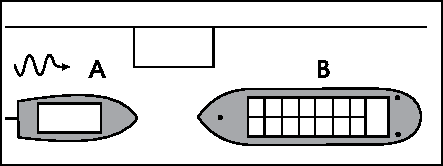
\includegraphics[width=\textwidth]{Hoofdstukken/Reglementen/pdf/engte_stroming.pdf}}	
		\label{pic:engte:1}
	\end{minipage}
	\hfill
\end{figure}
\vspace{-0.7cm}

\begin{figure}[H]
	\centering
	\begin{minipage}[t]{0.70\textwidth}
		\textbf{2.} Grote schepen hebben voorrang op kleine schepen.\\
		\textit{Het grote motorschip B heeft voorrang op het kleine motorschip A}
	\end{minipage}
	\hfill
	\begin{minipage}[t]{0.25\textwidth}
		\raisebox{-0.55\height}{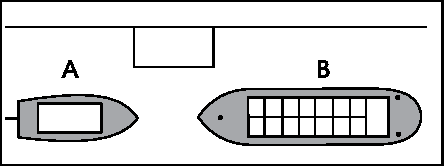
\includegraphics[width=\textwidth]{Hoofdstukken/Reglementen/pdf/engte_groot_klein.pdf}}	
		\label{pic:engte:2}
	\end{minipage}
	\hfill
\end{figure}
\vspace{-0.5cm}

\textbf{3.} Bij twee verschillende soorten schepen geldt de volgende volgorde van prioriteit. Een schip heeft voorrang op ieder ander schip met een lagere prioriteit.
\vspace{-0.5cm}
\begin{figure}[H]
	\centering
	\hspace{0.02\textwidth}
	\begin{minipage}[t]{0.70\textwidth}
		\textbf{1}. Een zeilschip welke de engte bezeilt\footnotemark. \\
		\textit{Het zeilschip A (bezeild de engte) gaat voor op de roeiboot}
	\end{minipage}
	\hfill
	\begin{minipage}[t]{0.25\textwidth}
		\raisebox{-0.55\height}{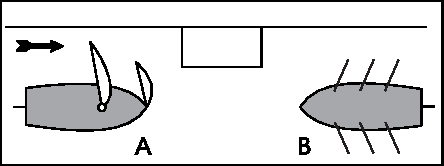
\includegraphics[width=\textwidth]{Hoofdstukken/Reglementen/pdf/engte_bezeild_spier.pdf}}	
		\label{pic:engte:3}
	\end{minipage}
	\hfill
\end{figure}
\footnotetext{Een bezeild punt kan bereikt worden zonder opkruisen}
\vspace{-0.7cm}

\begin{figure}[H]
	\centering
	\hspace{0.02\textwidth}
	\begin{minipage}[t]{0.70\textwidth}
		\textbf{2.} Een door spierkracht voortbewogen schip.\\
		\textit{Roeiboot A heeft voorrang op het motorschip B}
	\end{minipage}
	\hfill
	\begin{minipage}[t]{0.25\textwidth}
		\raisebox{-0.55\height}{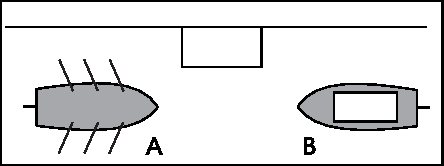
\includegraphics[width=\textwidth]{Hoofdstukken/Reglementen/pdf/engte_spier_motor.pdf}}	
		\label{pic:engte:4}
	\end{minipage}
	\hfill
\end{figure}

\vspace{-0.7cm}

\begin{figure}[H]
	\centering
	\hspace{0.02\textwidth}
	\begin{minipage}[t]{0.70\textwidth}
		\textbf{3.} Een motorschip.\\
		\textit{Het motorschip A gaat voor op het zeilschip B (bezeilt de engte niet)}
	\end{minipage}
	\hfill
	\begin{minipage}[t]{0.25\textwidth}
		\raisebox{-0.55\height}{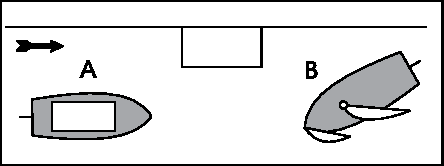
\includegraphics[width=\textwidth]{Hoofdstukken/Reglementen/pdf/engte_motor_niet_bezeild.pdf}}	
		\label{pic:engte:5}
	\end{minipage}
	\hfill
\end{figure}

\vspace{-0.7cm}

\begin{figure}[H]
	\centering
	\hspace{0.02\textwidth}
	\begin{minipage}[t]{0.70\textwidth}
		\textbf{4.} Een zeilschip welke de engte \textit{niet} bezeilt.\\
		\textit{Het zeilschip B gaat voor op het zeilschip A (bezeilt de engte niet)}
	\end{minipage}
	\hfill
	\begin{minipage}[t]{0.25\textwidth}
		\raisebox{-0.55\height}{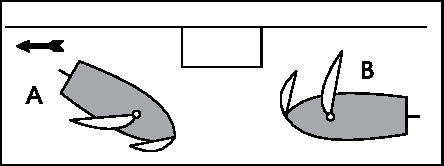
\includegraphics[width=\textwidth]{Hoofdstukken/Reglementen/pdf/engte_niet_bezeild_bezeild.pdf}}	
		\label{pic:engte:6}
	\end{minipage}
	\hfill
\end{figure}
\vspace{-0.7cm}
\begin{figure}[H]
	\centering
	\begin{minipage}[t]{0.70\textwidth}
		\textbf{4.} Zeilschepen onderling: Een zeilschip met zeilen over bakboord heeft voorrang.\\
		\textit{Zeilschip B (met zijn zeilen over bakboord) heeft voorrang op A}
	\end{minipage}
	\hfill
	\begin{minipage}[t]{0.25\textwidth}
		\raisebox{-0.75\height}{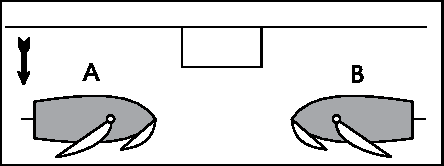
\includegraphics[width=\textwidth]{Hoofdstukken/Reglementen/pdf/engte_zeil_onderling.pdf}}	
		\label{pic:tegen:7}
	\end{minipage}
	\hfill
\end{figure}
\vspace{-0.5cm}
\textbf{5.} Roei- of motorschepen onderling:
\vspace{-0.5cm}
\begin{figure}[H]
	\centering
	\hspace{0.02\textwidth}
	\begin{minipage}[t]{0.70\textwidth}
		\textbf{5.1}. Het schip met de blokkade aan stuurboordswal verleent voorrang.\\
		\textit{Schip B (blokkade aan stuurboord) verleent voorrang aan schip A}
	\end{minipage}
	\hfill
	\begin{minipage}[t]{0.25\textwidth}
		\raisebox{-0.55\height}{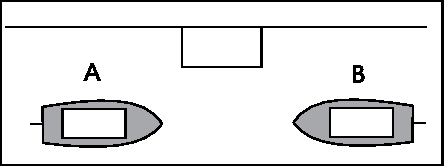
\includegraphics[width=\textwidth]{Hoofdstukken/Reglementen/pdf/engte_spier_motor_onderling.pdf}}	
		\label{pic:engte:9}
	\end{minipage}
	\hfill
\end{figure}

\vspace{-0.7cm}

\begin{figure}[H]
	\centering
	\hspace{0.02\textwidth}
	\begin{minipage}[t]{0.70\textwidth}
		\textbf{5.2} Het schip met de binnenbocht aan stuurboord verleent voorrang.\\
		\textit{Schip A (binnenbocht aan stuurboord) geeft voorrang aan schip B}
	\end{minipage}
	\hfill
	\begin{minipage}[t]{0.25\textwidth}
		\raisebox{-0.55\height}{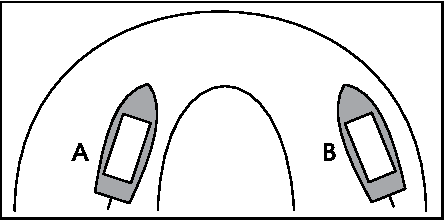
\includegraphics[width=\textwidth]{Hoofdstukken/Reglementen/pdf/engte_bocht_spier_motor.pdf}}	
		\label{pic:engte:10}
	\end{minipage}
	\hfill
\end{figure}
\vspace{-0.6cm}
\textit{Overige engtes met gelijke schepen vallen onder het goed zeemanschap.}

\paragraph{Oplopen}
Oplopen is \textit{enkel} toegestaan wanneer dit gedaan kan worden zonder gevaar voor andere schepen. Oplopen wordt voornamelijk langs bakboord gedaan. Het is echter ook toegestaan, wanneer de situatie hier om vraagt, om langs stuurboord op te lopen.



\begin{figure}[H]
	\centering
	\begin{minipage}[t]{0.70\textwidth}
	Zeilschepen onderling lopen elkaar op via de loefzijde. Hierdoor neem je de wind uit de zeilen van het opgelopen schip en gaat het oplopen sneller. Tijdens het oplopen mag medewerking verlangd worden van het opgelopen schip.
	\end{minipage}
	\hfill
	\begin{minipage}[t]{0.25\textwidth}
		\raisebox{-0.8\height}{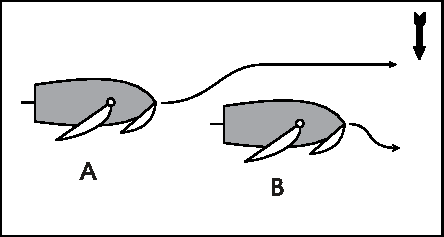
\includegraphics[width=\textwidth]{Hoofdstukken/Reglementen/pdf/oplopen.pdf}}
		\label{pic:op}
	\end{minipage}
	\hfill
\end{figure}

\subsection{Speciale manoeuvres}
Een schip mag enkel keren, vertrekken, een haven in- of uitvaren of een vaarwater oversteken wanneer dit zonder gevaar voor andere schepen kan. Het schip mag tijdens een van deze speciale manoeuvres medewerking verlangen van andere schepen, maar heeft \textit{geen} voorrang. Een uitzondering hierop geldt voor grote schepen. Wanneer deze een speciale manoeuvre maken zijn kleine schepen verplicht voorrang te geven.

\subsection{Voorrangsregels op een rij}
Om de voorrangsregels makkelijk te kunnen onthouden staan ze hieronder samengevat:\\[0.1cm]
Bij \textbf{kruisende koersen} kijk je naar de volgende regels:
\vspace*{-0.15cm}
\begin{enumerate}
    \item Het stuurboordswal varende schip gaat voor
    \item Grote schepen gaan voor op kleine schepen
    \item Hoofdwater gaat voor nevenwater
    \item Zeilschip gaat voor roeiboot gaat voor motorschip
    \item Roei- of motorschepen onderling: het schip van rechts gaat voor
    \item Zeilschepen onderling: 
        \stepcounter{enumi}
        \begin{enumerate}
	            \item [1.]Zeilen over bakboord gaat voor
	            \item [2.]Loef wijkt voor lij
	        \end{enumerate}
\end{enumerate}

Bij \textbf{tegengestelde koersen zonder engte} kijk je naar de volgende regels:
\vspace*{-0.15cm}
\begin{enumerate}
    \item Het stuurboordswal varende schip gaat voor
    \item Grote schepen gaan voor op kleine schepen
    \item Zeilschip gaat voor roeiboot gaat voor motorschip
    \item Zeilschepen onderling: zeilen over bakboord gaat voor
    \item Roei- of motorschepen onderling: beiden wijken naar bakboord
\end{enumerate}

Bij \textbf{tegengestelde koersen met engte} kijk je naar de volgende regels:
\vspace*{-0.15cm}
\begin{enumerate}
	\item Bij stroming heeft het schip wat met de stroom mee vaart voorrang
	\item Grote schepen gaan voor op kleine schepen
	\item Volgorde van prioriteit bij twee verschillende schepen:
	        \begin{enumerate}
					\item [1.] Een zeilschip die de engte bezeilt
					\item [2.] Een door spier voortbewogen schip
					\item [3.] Een motorschip
					\item [4.] Een zeilschip die de engte \textit{niet} bezeilt
					\end{enumerate}
	\item Zeilschepen onderling: zeilen over bakboord gaat voor 
	\item Roei- of motorschepen onderling: Het schip met de blokkade of binnenbocht aan stuurboord verleent voorrang

\end{enumerate}

Bij \textbf{oplopende koersen}, wijkt de oploper uit. Het opgelopen schip kan indien nodig uitwijken.

\section{Verkeerstekens}
Net als in het reguliere verkeer wordt er op het water gebruik gemaakt van verkeerstekens. In het BPR worden deze tekens gedefinieerd en onderverdeeld in een aantal groepen. In de onderstaande twee paragrafen staan de belangrijkste van deze tekens geïllustreerd samen met een toelichting.

\subsubsection*{Geboden en verplichtingen}
\begin{table}[H]
	\centering
	\begin{tabular}{cm{4.6cm}cm{4.6cm}}
	\raisebox{-0.5\height}{
\includegraphics[width=2cm]{Hoofdstukken/Reglementen/pdf/A1.pdf}} & In-, uit-, of doorvaren verboden &	\raisebox{-0.5\height}{
\includegraphics[width=2cm]{Hoofdstukken/Reglementen/pdf/A9.pdf}} & Verboden hinderlijke waterbeweging te veroorzaken  \\[1cm] %%%
	
	\raisebox{-0.5\height}{
\includegraphics[width=2cm]{Hoofdstukken/Reglementen/pdf/A12.pdf}} & Verboden voor motorschepen &	\raisebox{-0.5\height}{
\includegraphics[width=2cm]{Hoofdstukken/Reglementen/pdf/A13.pdf}} & Verboden voor kleine schepen  \\[1cm] %%% 
	
	\raisebox{-0.5\height}{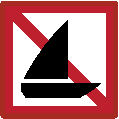
\includegraphics[width=2cm]{Hoofdstukken/Reglementen/pdf/A15.pdf}} & Verboden voor zeilschepen &	\raisebox{-0.5\height}{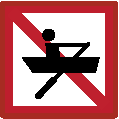
\includegraphics[width=2cm]{Hoofdstukken/Reglementen/pdf/A16.pdf}} & Verboden voor door spierkracht voortbewogen schepen  \\[1cm] %%% 
	
	\raisebox{-0.5\height}{
\includegraphics[width=2cm]{Hoofdstukken/Reglementen/pdf/A17.pdf}} & Verboden voor zeilplanken &	\raisebox{-0.5\height}{
\includegraphics[width=2cm]{Hoofdstukken/Reglementen/pdf/B5.pdf}} & Verplichting voor het bord stil te houden \\[1cm] %%% 
	
	\raisebox{-0.5\height}{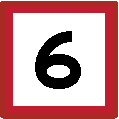
\includegraphics[width=2cm]{Hoofdstukken/Reglementen/pdf/B6.pdf}} & Verplichting de vaarsnelheid te beperken (in km/h)
	& &  %%% 
	\end{tabular}
\end{table}
\newpage

\subsubsection*{Aanwijzingstekens}
\begin{table}[H]
	\centering
	\begin{tabular}{cm{4.6cm}cm{4.6cm}}
		\raisebox{-0.5\height}{
\includegraphics[width=2cm]{Hoofdstukken/Reglementen/pdf/E4a.pdf}} & Niet vrijvarende veerpont
		 &	\raisebox{-0.5\height}{
\includegraphics[width=2cm]{Hoofdstukken/Reglementen/pdf/E4b.pdf}} & Vrijvarende veerpont  \\[1cm] %%%
		
		\raisebox{-0.5\height}{
\includegraphics[width=2cm]{Hoofdstukken/Reglementen/pdf/E9.pdf}} & Het gevolgde vaarwater geldt als hoofdvaarwater &	\raisebox{-0.5\height}{
\includegraphics[width=2cm]{Hoofdstukken/Reglementen/pdf/E10.pdf}} & Het gevolgde vaarwater geldt als nevenvaarwater  \\[1cm] %%% 
		
		\raisebox{-0.5\height}{
\includegraphics[width=2cm]{Hoofdstukken/Reglementen/pdf/E11.pdf}} & Einde van een verbod of gebod &	\raisebox{-0.5\height}{
\includegraphics[width=2cm]{Hoofdstukken/Reglementen/pdf/E15.pdf}} & Motorschepen toegestaan \\[1cm] %%% 
		
		\raisebox{-0.5\height}{
\includegraphics[width=2cm]{Hoofdstukken/Reglementen/pdf/E16.pdf}} & Kleine schepen toegestaan &	\raisebox{-0.5\height}{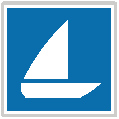
\includegraphics[width=2cm]{Hoofdstukken/Reglementen/pdf/E18.pdf}} & Zeilschepen toegestaan\\[1cm] %%% 
		
		\raisebox{-0.5\height}{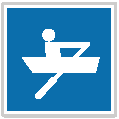
\includegraphics[width=2cm]{Hoofdstukken/Reglementen/pdf/E19.pdf}} & Door spierkracht voortbewogen schepen toegestaan &	\raisebox{-0.5\height}{
\includegraphics[width=2cm]{Hoofdstukken/Reglementen/pdf/E20.pdf}} & Zeilplanken toegestaan \\[1cm] %%% 
	\end{tabular}
\end{table}


\section{Geluidsseinen}
Om te kunnen communiceren met andere schepen op het water zijn een aantal standaard geluidssignalen gedefinieerd in het BPR. Deze signalen kunnen door middel van een scheepshoorn of andere geluidsinstallatie gegeven worden.  
Alle grote schepen en kleine gemotoriseerde schepen dienen deze geluidssignalen te kunnen maken. 

Een signaal is opgebouwd uit lange stoten (4 seconden) en korte stoten (1 seconden). Tussen opvolgende stoten zit één korte stoot pauze. De signalen en hun betekenis staan in tabel \ref{tab:geluid}.

\newcommand{\sshort}{\rule{2mm}{2mm}} %Signal short
\newcommand{\slong}{\rule{6mm}{2mm}}  %Signal long
\newcommand{\sspace}{\hspace{2mm}}  %Signal space


\begin{table}[h]
	\centering
	\caption{Geluidssignalen}
	\label{tab:geluid}
	\begin{tabular}{l|l}
		\textbf{Betekenis} & \textbf{Signaal} \\ \hline
		Attentie & \slong  \\
		Ik ga stuurboord uit & \sshort \\
		Ik ga bakboord uit & \sshort \sspace \sshort \\
		Ik sla achteruit & \sshort \sspace \sshort \sspace \sshort \\
		Ik kan niet manoeuvreren & \sshort \sspace \sshort \sspace \sshort \sspace \sshort \\
		Noodsein & \slong \sspace  \slong \sspace  \slong \sspace (reeks)  \\
		Blijf weg sein\footnotemark & \sshort \sspace \slong \sspace \sshort \sspace \slong \sspace  \sshort \sspace \slong \sspace (reeks)  \\
		Verzoek tot bediening van brug of sluis & \slong \sspace  \sshort \sspace  \slong
	\end{tabular}
\end{table}

\footnotetext{Het blijf-weg-sein wordt alleen gegeven door schepen met een gevaarlijke lading}

\section{Overige regels}
\subsubsection*{Hinderlijke vaarbewegingen}
Om schade en overlast bij andere schepen te voorkomen is het verplicht bij sommige locaties op het water de snelheid dusdanig te minderen om hinderingen te voorkomen. Dit gaat om havenmondingen, afgemeerde schepen en veerpoten. Daarnaast zijn er een aantal borden en lichtseinen die een hinderlijke vaarbewegingen verbieden.



\subsubsection*{Motorplicht}
Op een aantal vaarwateren in Nederland geldt voor kleine schepen de verplichting dat deze een gebruiksklare motor moeten hebben waarmee minimaal 6 km/h gevaren kan worden. Dit komt omdat dit drukke wateren zijn met veel beroepsvaart. De kleine schepen moeten zoveel mogelijk stuurboordswal varen en voor zeilschepen is het hier niet toegestaan op te kruisen. De wateren staan in bijlage 15 van het BPR en zijn tevens hieronder genoteerd:

\begin{itemize}
	\begin{multicols}{2}
	\item het Noordzeekanaal;
	\item de Noord;
	\item de Oude Maas;
	\item de Dordtsche Kil;
	\item het Kanaal door Zuid-Beveland;
	\item het Brabantsche Vaarwater;
	\item de Witte Tonnen Vlije;
	\item de Schelde-Rijnverbinding;
	\item het Kanaal van Sint Andries;
	\item de Boven-Merwede;
	\item de Beneden-Merwede;
	\item het Julianakanaal;
	\item de Waal;
	\item de Boven-Rijn;
	\item het Pannerdensch Kanaal;
	\item de Neder-Rijn tot kmr 886;
	\item het Amsterdam-Rijnkanaal;
	\item het Lekkanaal;
	\item het betonde vaarwater van het Buiten-IJ;
	\item het Afgesloten-IJ;
	\item de Nieuwe Maas;
	\item het Scheur;
	\item de Nieuwe Waterweg;
	\item de Maasmond;
	\item het Calandkanaal;
	\item het Beerkanaal;
	\item de Koningshaven;
	\item het Zuiddiepje;
	\item de Veerhaven te Terneuzen;
	\item het Prinses Margrietkanaal;
	\item het Van Starkenborghkanaal;
	\item het Eemskanaal;
	\end{multicols}
	\item De vaarweg ten westen van de Noordzeesluizen te IJmuiden, met inbegrip van de daaraan gelegen havens;
	\item de Geldersche IJssel vanaf de IJsselkop tot aan de monding van het Twenthekanaal;
	\item de Gekanaliseerde Maas van Maastricht (kmr 12,000) tot Borgharen;
	\item het betonde hoofdvaarwater van de Nieuwe Merwede;
	\item het betonde hoofdvaarwater van het Hollandsch Diep;
\end{itemize}

\section{Conclusie}
Na het lezen van dit hoofdstuk heb je verstand van de voorrangsregels op het water. Een van de belangrijkste is het goed zeemanschap, wat inhoudt dat je alles doet om een gevaarlijke situatie of aanvaring te voorkomen. Daarnaast ken je de verschillende voorrangssituaties en volgorde en weet je hoe je de regels moet toepassen. 